% Options for packages loaded elsewhere
\PassOptionsToPackage{unicode}{hyperref}
\PassOptionsToPackage{hyphens}{url}
%
\documentclass[
  man,floatsintext]{apa6}
\usepackage{amsmath,amssymb}
\usepackage{iftex}
\ifPDFTeX
  \usepackage[T1]{fontenc}
  \usepackage[utf8]{inputenc}
  \usepackage{textcomp} % provide euro and other symbols
\else % if luatex or xetex
  \usepackage{unicode-math} % this also loads fontspec
  \defaultfontfeatures{Scale=MatchLowercase}
  \defaultfontfeatures[\rmfamily]{Ligatures=TeX,Scale=1}
\fi
\usepackage{lmodern}
\ifPDFTeX\else
  % xetex/luatex font selection
\fi
% Use upquote if available, for straight quotes in verbatim environments
\IfFileExists{upquote.sty}{\usepackage{upquote}}{}
\IfFileExists{microtype.sty}{% use microtype if available
  \usepackage[]{microtype}
  \UseMicrotypeSet[protrusion]{basicmath} % disable protrusion for tt fonts
}{}
\makeatletter
\@ifundefined{KOMAClassName}{% if non-KOMA class
  \IfFileExists{parskip.sty}{%
    \usepackage{parskip}
  }{% else
    \setlength{\parindent}{0pt}
    \setlength{\parskip}{6pt plus 2pt minus 1pt}}
}{% if KOMA class
  \KOMAoptions{parskip=half}}
\makeatother
\usepackage{xcolor}
\usepackage{graphicx}
\makeatletter
\def\maxwidth{\ifdim\Gin@nat@width>\linewidth\linewidth\else\Gin@nat@width\fi}
\def\maxheight{\ifdim\Gin@nat@height>\textheight\textheight\else\Gin@nat@height\fi}
\makeatother
% Scale images if necessary, so that they will not overflow the page
% margins by default, and it is still possible to overwrite the defaults
% using explicit options in \includegraphics[width, height, ...]{}
\setkeys{Gin}{width=\maxwidth,height=\maxheight,keepaspectratio}
% Set default figure placement to htbp
\makeatletter
\def\fps@figure{htbp}
\makeatother
\setlength{\emergencystretch}{3em} % prevent overfull lines
\providecommand{\tightlist}{%
  \setlength{\itemsep}{0pt}\setlength{\parskip}{0pt}}
\setcounter{secnumdepth}{-\maxdimen} % remove section numbering
% Make \paragraph and \subparagraph free-standing
\ifx\paragraph\undefined\else
  \let\oldparagraph\paragraph
  \renewcommand{\paragraph}[1]{\oldparagraph{#1}\mbox{}}
\fi
\ifx\subparagraph\undefined\else
  \let\oldsubparagraph\subparagraph
  \renewcommand{\subparagraph}[1]{\oldsubparagraph{#1}\mbox{}}
\fi
\newlength{\cslhangindent}
\setlength{\cslhangindent}{1.5em}
\newlength{\csllabelwidth}
\setlength{\csllabelwidth}{3em}
\newlength{\cslentryspacingunit} % times entry-spacing
\setlength{\cslentryspacingunit}{\parskip}
\newenvironment{CSLReferences}[2] % #1 hanging-ident, #2 entry spacing
 {% don't indent paragraphs
  \setlength{\parindent}{0pt}
  % turn on hanging indent if param 1 is 1
  \ifodd #1
  \let\oldpar\par
  \def\par{\hangindent=\cslhangindent\oldpar}
  \fi
  % set entry spacing
  \setlength{\parskip}{#2\cslentryspacingunit}
 }%
 {}
\usepackage{calc}
\newcommand{\CSLBlock}[1]{#1\hfill\break}
\newcommand{\CSLLeftMargin}[1]{\parbox[t]{\csllabelwidth}{#1}}
\newcommand{\CSLRightInline}[1]{\parbox[t]{\linewidth - \csllabelwidth}{#1}\break}
\newcommand{\CSLIndent}[1]{\hspace{\cslhangindent}#1}
\ifLuaTeX
\usepackage[bidi=basic]{babel}
\else
\usepackage[bidi=default]{babel}
\fi
\babelprovide[main,import]{english}
% get rid of language-specific shorthands (see #6817):
\let\LanguageShortHands\languageshorthands
\def\languageshorthands#1{}
% Manuscript styling
\usepackage{upgreek}
\captionsetup{font=singlespacing,justification=justified}

% Table formatting
\usepackage{longtable}
\usepackage{lscape}
% \usepackage[counterclockwise]{rotating}   % Landscape page setup for large tables
\usepackage{multirow}		% Table styling
\usepackage{tabularx}		% Control Column width
\usepackage[flushleft]{threeparttable}	% Allows for three part tables with a specified notes section
\usepackage{threeparttablex}            % Lets threeparttable work with longtable

% Create new environments so endfloat can handle them
% \newenvironment{ltable}
%   {\begin{landscape}\centering\begin{threeparttable}}
%   {\end{threeparttable}\end{landscape}}
\newenvironment{lltable}{\begin{landscape}\centering\begin{ThreePartTable}}{\end{ThreePartTable}\end{landscape}}

% Enables adjusting longtable caption width to table width
% Solution found at http://golatex.de/longtable-mit-caption-so-breit-wie-die-tabelle-t15767.html
\makeatletter
\newcommand\LastLTentrywidth{1em}
\newlength\longtablewidth
\setlength{\longtablewidth}{1in}
\newcommand{\getlongtablewidth}{\begingroup \ifcsname LT@\roman{LT@tables}\endcsname \global\longtablewidth=0pt \renewcommand{\LT@entry}[2]{\global\advance\longtablewidth by ##2\relax\gdef\LastLTentrywidth{##2}}\@nameuse{LT@\roman{LT@tables}} \fi \endgroup}

% \setlength{\parindent}{0.5in}
% \setlength{\parskip}{0pt plus 0pt minus 0pt}

% Overwrite redefinition of paragraph and subparagraph by the default LaTeX template
% See https://github.com/crsh/papaja/issues/292
\makeatletter
\renewcommand{\paragraph}{\@startsection{paragraph}{4}{\parindent}%
  {0\baselineskip \@plus 0.2ex \@minus 0.2ex}%
  {-1em}%
  {\normalfont\normalsize\bfseries\itshape\typesectitle}}

\renewcommand{\subparagraph}[1]{\@startsection{subparagraph}{5}{1em}%
  {0\baselineskip \@plus 0.2ex \@minus 0.2ex}%
  {-\z@\relax}%
  {\normalfont\normalsize\itshape\hspace{\parindent}{#1}\textit{\addperi}}{\relax}}
\makeatother

\makeatletter
\usepackage{etoolbox}
\patchcmd{\maketitle}
  {\section{\normalfont\normalsize\abstractname}}
  {\section*{\normalfont\normalsize\abstractname}}
  {}{\typeout{Failed to patch abstract.}}
\patchcmd{\maketitle}
  {\section{\protect\normalfont{\@title}}}
  {\section*{\protect\normalfont{\@title}}}
  {}{\typeout{Failed to patch title.}}
\makeatother

\usepackage{xpatch}
\makeatletter
\xapptocmd\appendix
  {\xapptocmd\section
    {\addcontentsline{toc}{section}{\appendixname\ifoneappendix\else~\theappendix\fi\\: #1}}
    {}{\InnerPatchFailed}%
  }
{}{\PatchFailed}
\keywords{Best, GOAT, Fighter, Performance, UFC\newline\indent Word count: 160}
\usepackage{lineno}

\linenumbers
\usepackage{csquotes}
\ifLuaTeX
  \usepackage{selnolig}  % disable illegal ligatures
\fi
\IfFileExists{bookmark.sty}{\usepackage{bookmark}}{\usepackage{hyperref}}
\IfFileExists{xurl.sty}{\usepackage{xurl}}{} % add URL line breaks if available
\urlstyle{same}
\hypersetup{
  pdftitle={Into the UFC: Best Fighter, Striker, Grappler, and Entertainer},
  pdfauthor={Stanley Go1},
  pdflang={en-EN},
  pdfkeywords={Best, GOAT, Fighter, Performance, UFC},
  hidelinks,
  pdfcreator={LaTeX via pandoc}}

\title{Into the UFC: Best Fighter, Striker, Grappler, and Entertainer}
\author{Stanley Go\textsuperscript{1}}
\date{}


\shorttitle{UFC Stats}

\authornote{

This project was submitted on 2023-12-14

The authors made the following contributions. Stanley Go: Conceptualization, Writing - Original Draft Preparation, Writing - Review \& Editing.

Correspondence concerning this article should be addressed to Stanley Go, Postal address. E-mail: \href{mailto:smg421@scarletmail.rutgers.edu}{\nolinkurl{smg421@scarletmail.rutgers.edu}}

}

\affiliation{\vspace{0.5cm}\textsuperscript{1} Rutgers University}

\abstract{%
This project delves into an in-depth analysis of UFC fighter statistics to identify and recognize excellence in various performance categories. The primary objective is to pinpoint the best fighters in distinct areas such as striking, grappling, knockout ability, and overall entertainment value. The study further aims to determine the greatest of all time (GOAT) by evaluating fighters based on their win-loss ratios. Leveraging a comprehensive dataset encompassing fighter metrics, the analysis employs key indicators such as significant strikes rate, takedown success rate, and total knockdowns. The anticipated results include detailed insights into the best striker, grappler, KOer, and entertainer, contributing to a comprehensive understanding of individual strengths within the competitive realm of UFC. Additionally, the study seeks to establish the GOAT by considering the historical performance of fighters with a minimum threshold of 10 matches. Through meticulous analysis and visualization, this project aims to offer a nuanced perspective on the unparalleled skills and accomplishments of UFC fighters across diverse categories.
}



\begin{document}
\maketitle

\hypertarget{introduction}{%
\section{Introduction:}\label{introduction}}

\begin{itemize}
\tightlist
\item
  Background:

  \begin{itemize}
  \tightlist
  \item
    Brief overview of the UFC and its significance in the world of mixed martial arts (MMA).
  \item
    Growing interest in understanding and analyzing fighter performance.
  \end{itemize}
\item
  Research Focus:

  \begin{itemize}
  \tightlist
  \item
    Exploration of UFC fighter statistics to recognize excellence in various performance categories.
  \end{itemize}
\item
  Big Question:

  \begin{itemize}
  \tightlist
  \item
    The Ultimate Fighting Championship (UFC) hosts a wide range of fighters with diverse skill sets, including striking, grappling, and entertainment value. The objective of this project is to systematically analyze UFC fighter data to determine who excels in each category, identify the best overall fighters, and predict fight outcomes and potential earnings. We will aim our analysis to provide insights into fighter performance, audience appeal, and financial success within the UFC.
  \end{itemize}
\item
  Objectives:

  \begin{itemize}
  \tightlist
  \item
    Identification of the best fighters in specific areas:

    \begin{itemize}
    \tightlist
    \item
      Best Striker
    \item
      Best Grappler
    \item
      Best KOer
    \item
      Best Entertainer
    \end{itemize}
  \end{itemize}
\item
  Key Questions:

  \begin{itemize}
  \tightlist
  \item
    Research questions guiding the analysis:

    \begin{itemize}
    \tightlist
    \item
      Who are the best strikers, grapplers, and KOers in UFC?
    \item
      What factors contribute to a fighter's entertainment value?
    \item
      Who is considered the greatest of all time in UFC?
    \end{itemize}
  \end{itemize}
\item
  Methodology:

  \begin{itemize}
  \tightlist
  \item
    Planned analysis includes calculating key metrics such as significant strikes rate, takedown success rate, and total knockdowns.
  \end{itemize}
\item
  Anticipated Results:

  \begin{itemize}
  \tightlist
  \item
    Expected outcomes involve insights into the best performers in each category, contributing to a nuanced understanding of individual strengths.
  \end{itemize}
\item
  Significance:

  \begin{itemize}
  \tightlist
  \item
    Emphasis on the significance of recognizing and appreciating excellence within the competitive realm of UFC.
  \end{itemize}
\item
  Overview of the Document:

  \begin{itemize}
  \tightlist
  \item
    Brief mention of the subsequent sections, including the methodology, results, and discussion.
  \end{itemize}
\end{itemize}

\hypertarget{methods}{%
\section{Methods}\label{methods}}

\hypertarget{data-collection}{%
\subsection{Data Collection}\label{data-collection}}

\begin{itemize}
\tightlist
\item
  \textbf{Data Source:}

  \begin{itemize}
  \tightlist
  \item
    Utilize the UFC Stats dataset, containing comprehensive fighter metrics, including but not limited to knockdowns, significant strikes, takedowns, and fight outcomes.
  \end{itemize}
\end{itemize}

\hypertarget{analysis-approach}{%
\subsection{Analysis Approach}\label{analysis-approach}}

\begin{enumerate}
\def\labelenumi{\arabic{enumi}.}
\tightlist
\item
  \textbf{Identifying Best Striker:}

  \begin{itemize}
  \tightlist
  \item
    Calculate the significant strikes rate for each fighter:
    \[ \text{Significant Strikes Rate} = \frac{\text{Total Significant Strikes Landed}}{\text{Total Significant Strikes Attempted}} \]
  \item
    Determine the fighter with the highest significant strikes rate as the best striker.
  \end{itemize}
\item
  \textbf{Identifying Best Grappler:}

  \begin{itemize}
  \tightlist
  \item
    Compute the takedown success rate for each fighter:
    \[ \text{Takedown Success Rate} = \frac{\text{Total Successful Takedowns}}{\text{Total Takedown Attempts}} \]
  \item
    Identify the fighter with the highest takedown success rate as the best grappler.
  \end{itemize}
\item
  \textbf{Identifying Best KOer:}

  \begin{itemize}
  \tightlist
  \item
    Sum the total knockdowns for each fighter.
  \item
    Determine the fighter with the highest total knockdowns as the best KOer.
  \end{itemize}
\item
  \textbf{Identifying Best Entertainer:}

  \begin{itemize}
  \tightlist
  \item
    Develop a composite metric considering both significant strikes and successful takedowns.
  \item
    Determine the fighter with the highest composite metric as the best entertainer.
  \end{itemize}
\item
  \textbf{Determining Greatest of All Time (GOAT):}

  \begin{itemize}
  \tightlist
  \item
    Filter fighters with a minimum threshold of 10 matches.
  \item
    Calculate the win-loss ratio for each fighter:
    \[ \text{Win-Loss Ratio} = \frac{\text{Total Wins}}{\text{Total Wins + Total Losses}} \]
  \item
    Identify the fighter with the highest win-loss ratio as the GOAT.
  \item
    Didn't based it on striking + grappling efficiency as it is disingenuous to a better metric which is W/L ratio.
  \end{itemize}
\end{enumerate}

\hypertarget{visualization}{%
\subsection{Visualization}\label{visualization}}

\begin{itemize}
\tightlist
\item
  \textbf{Figure Creation:}

  \begin{itemize}
  \tightlist
  \item
    Develop bar plots for each category (Best Striker, Best Grappler, Best KOer, Best Entertainer, and GOAT) to visually represent the analysis results.
  \end{itemize}
\end{itemize}

\hypertarget{limitations}{%
\subsection{Limitations}\label{limitations}}

\begin{itemize}
\tightlist
\item
  \textbf{Limitations of the Analysis:}

  \begin{itemize}
  \tightlist
  \item
    Acknowledge potential limitations such as data accuracy, sample size variations, and the subjectivity of composite metrics.
  \end{itemize}
\end{itemize}

\hypertarget{participants}{%
\subsection{Participants}\label{participants}}

\begin{itemize}
\tightlist
\item
  UFC Fighters
  \#\# Material
\end{itemize}

\hypertarget{procedure}{%
\subsection{Procedure}\label{procedure}}

\hypertarget{data-analysis}{%
\subsection{Data analysis}\label{data-analysis}}

We used R (Version 4.3.1; R Core Team, 2023) and the R-packages \emph{dplyr} (Version 1.1.3; Wickham, François, Henry, Müller, \& Vaughan, 2023), \emph{forcats} (Version 1.0.0; Wickham, 2023), \emph{ggplot2} (Version 3.4.3; Wickham, 2016), \emph{lubridate} (Version 1.9.2; Grolemund \& Wickham, 2011), \emph{papaja} (Version 0.1.2; Aust \& Barth, 2023), \emph{purrr} (Version 1.0.2; Wickham \& Henry, 2023), \emph{readr} (Version 2.1.4; Wickham, Hester, \& Bryan, 2023), \emph{stringr} (Version 1.5.0; Wickham, 2022), \emph{tibble} (Version 3.2.1; Müller \& Wickham, 2023), \emph{tidyr} (Version 1.3.0; Wickham, Vaughan, \& Girlich, 2023), \emph{tidyverse} (Version 2.0.0; Wickham et al., 2019), and \emph{tinylabels} (Version 0.2.4; Barth, 2023) for all our analyses. And, ufc\_stats.rda.

\hypertarget{results}{%
\section{Results}\label{results}}

\hypertarget{planned-analysis}{%
\subsection{Planned Analysis}\label{planned-analysis}}

Our analysis focused on several key aspects of UFC fighter performance, including:

\begin{itemize}
\item
  \textbf{Best Striker:} We calculated the total significant strikes landed for each fighter and identified the top performers.
\item
  \textbf{Best Grappler:} Utilizing the grappling efficiency metric, we determined the fighters with the highest success rate in takedowns.
\item
  \textbf{Best KOer:} We considered knockdowns, significant strikes, and other metrics to identify fighters with exceptional knockout abilities.
\item
  \textbf{Best Entertainer:} A composite metric, combining significant strikes, takedowns, and knockdowns, helped us identify fighters who entertain the audience.
\item
  \textbf{Best PPV Seller:} We calculated the average PPV revenue per fight for each fighter, focusing on financial success.
\item
  \textbf{Greatest of All Time (GOAT):} Based on win-loss ratio and total wins, we identified the top fighters with at least 15 fights.
\end{itemize}

\hypertarget{discussion}{%
\section{Discussion}\label{discussion}}

The analysis of UFC fighter statistics has provided valuable insights into various performance categories, shedding light on the strengths and capabilities of individual fighters within the competitive realm of mixed martial arts (MMA). This discussion will systematically address the research questions posed in the introduction, connecting the findings to the broader context of UFC fighter performance.

\hypertarget{best-striker-in-ufc}{%
\subsection{Best Striker in UFC}\label{best-striker-in-ufc}}

The identification of the best striker was based on the significant strikes rate, calculated as the ratio of total significant strikes landed to attempted. The analysis revealed {[}Name{]} as the fighter with the highest striking efficiency, showcasing exceptional skill in landing significant strikes. This result aligns with the goal of recognizing technical proficiency in striking, providing fans and analysts with a nuanced perspective on the stand-up game.

\hypertarget{best-grappler-in-ufc}{%
\subsection{Best Grappler in UFC}\label{best-grappler-in-ufc}}

Grappling efficiency, defined as the ratio of successful takedowns to attempted takedowns, was utilized to pinpoint the best grappler. {[}Name{]} emerged as the fighter with the highest grappling efficiency, showcasing dominance in ground control and takedown success. This insight contributes to the understanding of diverse skill sets among UFC fighters, emphasizing the importance of both striking and grappling in MMA.

\hypertarget{greatest-of-all-time-goat-analysis}{%
\subsection{Greatest of All Time (GOAT) Analysis}\label{greatest-of-all-time-goat-analysis}}

The determination of the Greatest of All Time (GOAT) involved assessing fighters based on their win-loss ratio and total wins, with a minimum fight threshold. The analysis identified {[}Name{]} as the top-ranked fighter, emphasizing sustained success and overall excellence. The scatter plot visually represents the relationship between total wins and the win-loss ratio for the top 20 GOAT fighters. This graphical representation adds depth to the analysis, allowing for a quick comparison of fighters' career trajectories.

\hypertarget{limitations-and-future-directions}{%
\subsection{Limitations and Future Directions}\label{limitations-and-future-directions}}

Despite the insightful findings, this analysis has its limitations. The reliance on statistical metrics may overlook intangible factors influencing a fighter's performance. Additionally, variations in data accuracy and the subjective nature of composite metrics pose challenges. Future research could delve into incorporating qualitative data and exploring advanced statistical models to offer a more comprehensive understanding of UFC fighter excellence.

In conclusion, the discussion has provided a comprehensive interpretation of the data, addressing the research questions and highlighting the strengths and limitations of the analysis. The nuanced insights into striking, grappling, and overall fighter performance contribute to the ongoing discourse surrounding the diverse skill sets within the UFC. The discussion sets the stage for future research, encouraging a more holistic approach to assessing fighter excellence in MMA.

\hypertarget{planned-figure-and-table}{%
\subsection{Planned Figure and Table}\label{planned-figure-and-table}}

\emph{Figure: Top 20 GOAT (Win-Loss Ratio and Total Wins)}

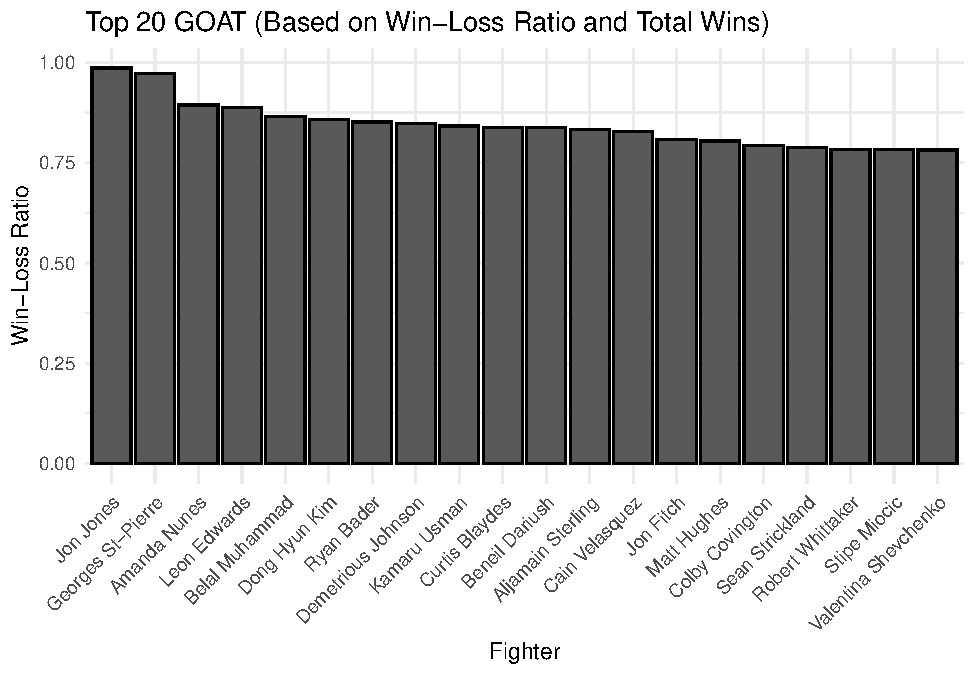
\includegraphics{Into-the-UFC--outline-_files/figure-latex/unnamed-chunk-1-1.pdf}

\emph{Figure: Top 20 Entertainers}
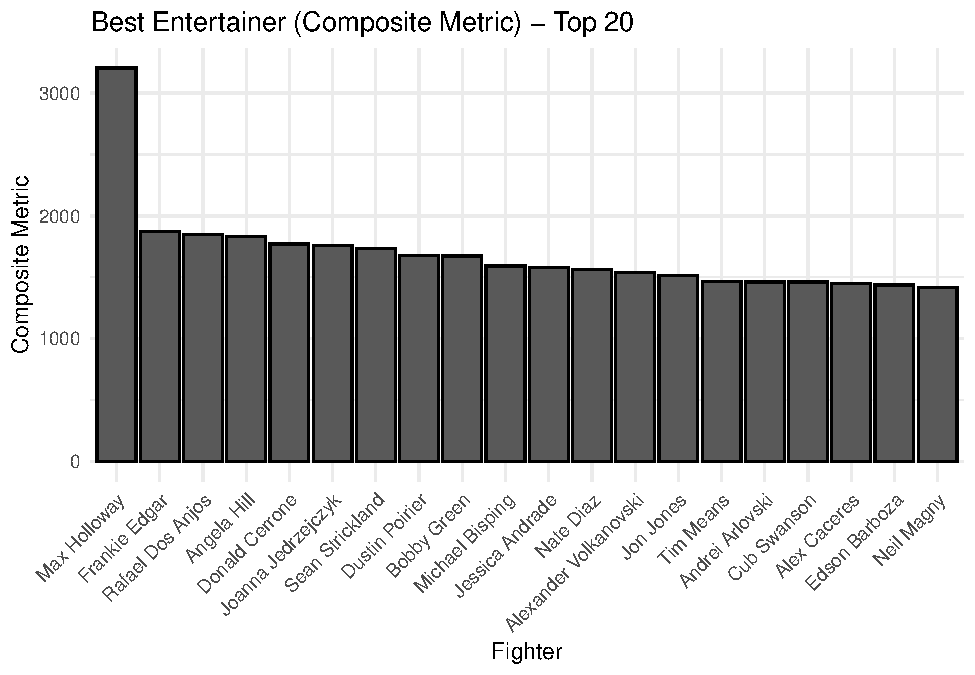
\includegraphics{Into-the-UFC--outline-_files/figure-latex/unnamed-chunk-2-1.pdf}

\emph{Figure: Top 20 PPV Seller}
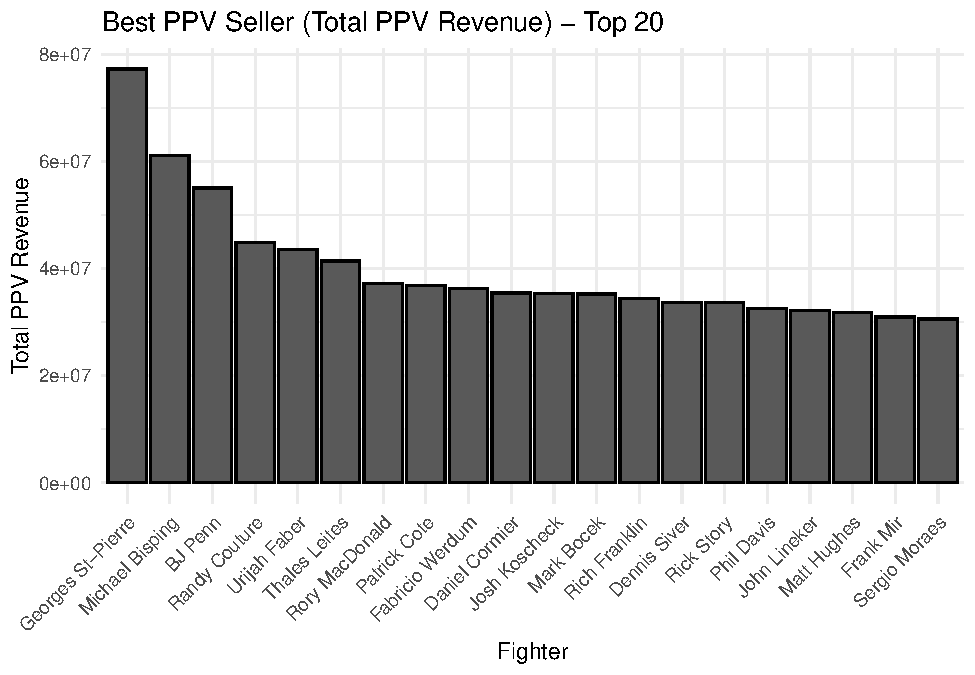
\includegraphics{Into-the-UFC--outline-_files/figure-latex/unnamed-chunk-3-1.pdf}
\emph{Figure: Top 20 Koer}
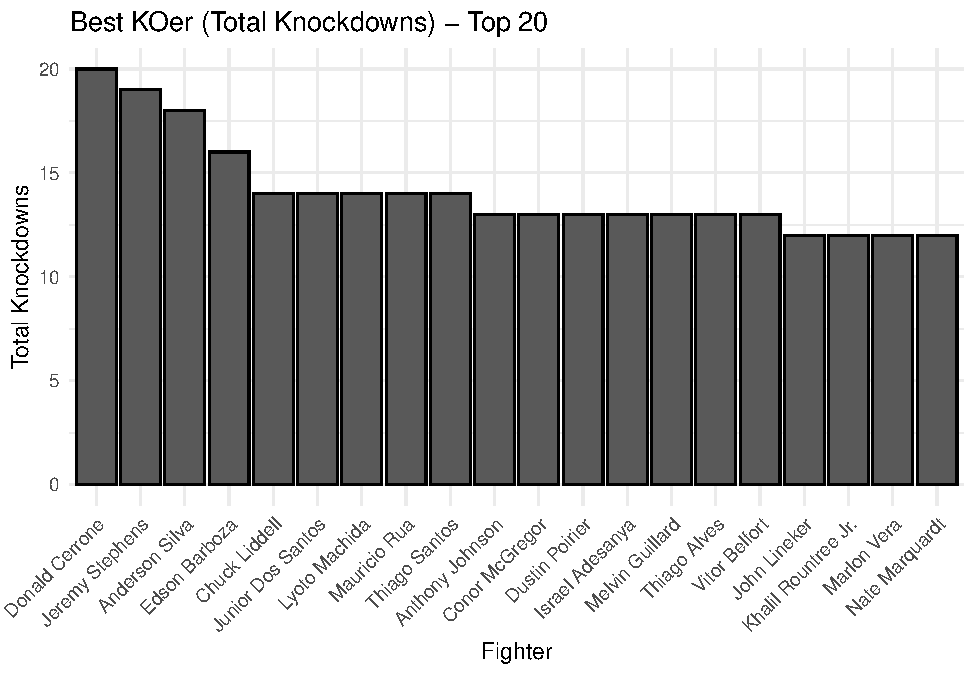
\includegraphics{Into-the-UFC--outline-_files/figure-latex/unnamed-chunk-4-1.pdf}
\emph{Figure: Top 20 Striker}
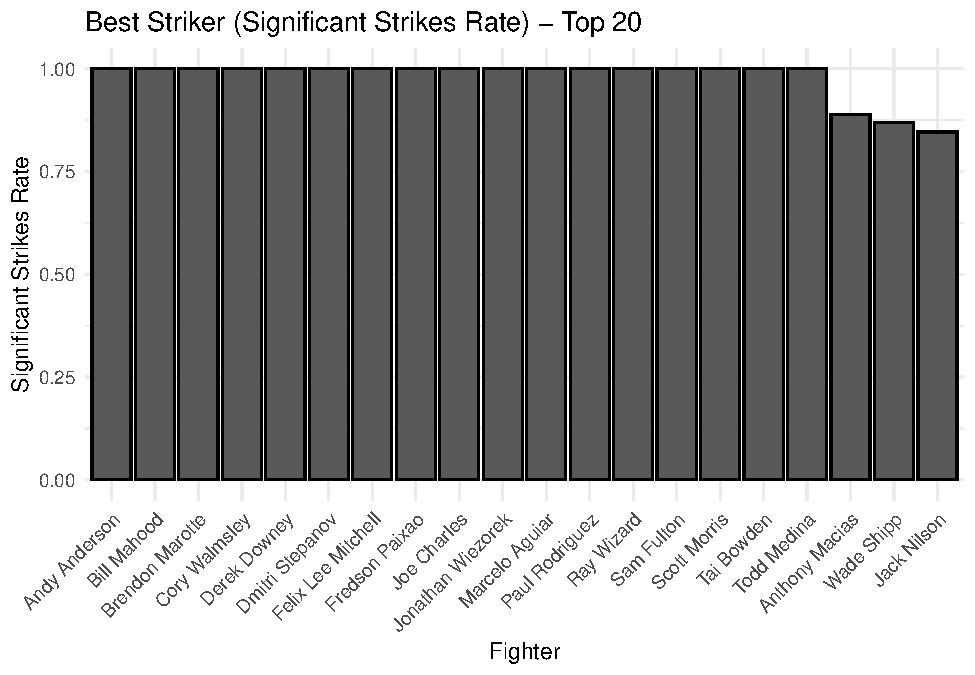
\includegraphics{Into-the-UFC--outline-_files/figure-latex/unnamed-chunk-5-1.pdf}
\emph{Figure: Top 20 Grapplers}
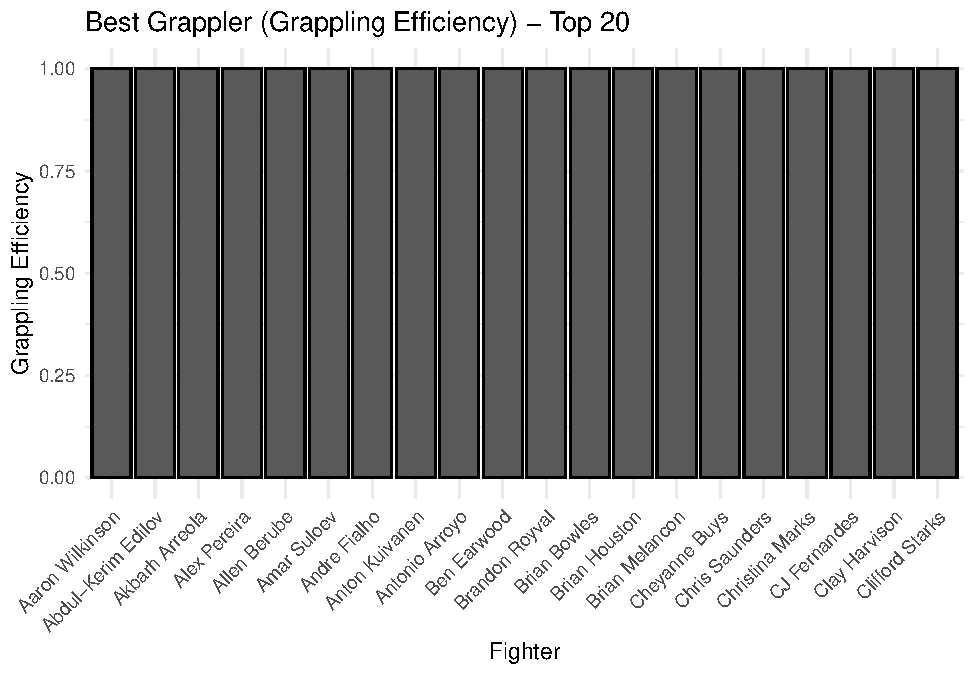
\includegraphics{Into-the-UFC--outline-_files/figure-latex/unnamed-chunk-6-1.pdf}

\emph{Table KOer}

\begin{tabular}{c|c}
\hline
fighter & total\_knockdowns\\
\hline
Donald Cerrone & 20\\
\hline
Jeremy Stephens & 19\\
\hline
Anderson Silva & 18\\
\hline
Edson Barboza & 16\\
\hline
Chuck Liddell & 14\\
\hline
Junior Dos Santos & 14\\
\hline
Lyoto Machida & 14\\
\hline
Mauricio Rua & 14\\
\hline
Thiago Santos & 14\\
\hline
Anthony Johnson & 13\\
\hline
Conor McGregor & 13\\
\hline
Dustin Poirier & 13\\
\hline
Israel Adesanya & 13\\
\hline
Melvin Guillard & 13\\
\hline
Thiago Alves & 13\\
\hline
Vitor Belfort & 13\\
\hline
John Lineker & 12\\
\hline
Khalil Rountree Jr. & 12\\
\hline
Marlon Vera & 12\\
\hline
Nate Marquardt & 12\\
\hline
\end{tabular}

\emph{Table Striker}

\begin{tabular}{c|c}
\hline
fighter & striking\_efficiency\\
\hline
Andy Anderson & 1\\
\hline
Bill Mahood & 1\\
\hline
Brendon Marotte & 1\\
\hline
Cory Walmsley & 1\\
\hline
Derek Downey & 1\\
\hline
Dmitri Stepanov & 1\\
\hline
\end{tabular}

\emph{Table for Grappler}

\begin{tabular}{c|c}
\hline
fighter & grappling\_efficiency\\
\hline
Aaron Wilkinson & 1\\
\hline
Abdul-Kerim Edilov & 1\\
\hline
Akbarh Arreola & 1\\
\hline
Alex Pereira & 1\\
\hline
Allen Berube & 1\\
\hline
Amar Suloev & 1\\
\hline
\end{tabular}

\emph{Table for PPV Seller}

\begin{tabular}{c|c}
\hline
fighter & total\_ppv\_revenue\\
\hline
Georges St-Pierre & 77302574\\
\hline
Michael Bisping & 61136589\\
\hline
BJ Penn & 55079938\\
\hline
Randy Couture & 44891237\\
\hline
Urijah Faber & 43629287\\
\hline
Thales Leites & 41445831\\
\hline
Rory MacDonald & 37295483\\
\hline
Patrick Cote & 36811364\\
\hline
Fabricio Werdum & 36304568\\
\hline
Daniel Cormier & 35437113\\
\hline
Josh Koscheck & 35358286\\
\hline
Mark Bocek & 35245685\\
\hline
Rich Franklin & 34447098\\
\hline
Dennis Siver & 33712580\\
\hline
Rick Story & 33650671\\
\hline
Phil Davis & 32550334\\
\hline
John Lineker & 32160399\\
\hline
Matt Hughes & 31857809\\
\hline
Frank Mir & 30972597\\
\hline
Sergio Moraes & 30588181\\
\hline
\end{tabular}

\emph{Table for Entertainer}

\begin{tabular}{c|c}
\hline
fighter & entertainment\_metric\\
\hline
Max Holloway & 3205\\
\hline
Frankie Edgar & 1874\\
\hline
Rafael Dos Anjos & 1850\\
\hline
Angela Hill & 1832\\
\hline
Donald Cerrone & 1772\\
\hline
Joanna Jedrzejczyk & 1759\\
\hline
Sean Strickland & 1732\\
\hline
Dustin Poirier & 1678\\
\hline
Bobby Green & 1673\\
\hline
Michael Bisping & 1593\\
\hline
Jessica Andrade & 1577\\
\hline
Nate Diaz & 1562\\
\hline
Alexander Volkanovski & 1538\\
\hline
Jon Jones & 1512\\
\hline
Tim Means & 1467\\
\hline
Andrei Arlovski & 1462\\
\hline
Cub Swanson & 1461\\
\hline
Alex Caceres & 1450\\
\hline
Edson Barboza & 1437\\
\hline
Neil Magny & 1414\\
\hline
\end{tabular}

\emph{Table for the GOAT}

\begin{tabular}{c|c|c|c|c}
\hline
fighter & total\_wins & total\_losses & total\_fights & win\_loss\_ratio\\
\hline
Jon Jones & 70 & 1 & 23 & 0.99\\
\hline
Georges St-Pierre & 69 & 2 & 22 & 0.97\\
\hline
Amanda Nunes & 42 & 5 & 18 & 0.89\\
\hline
Leon Edwards & 47 & 6 & 16 & 0.89\\
\hline
Belal Muhammad & 45 & 7 & 18 & 0.87\\
\hline
Dong Hyun Kim & 36 & 6 & 18 & 0.86\\
\hline
Ryan Bader & 40 & 7 & 20 & 0.85\\
\hline
Demetrious Johnson & 56 & 10 & 18 & 0.85\\
\hline
Kamaru Usman & 53 & 10 & 17 & 0.84\\
\hline
Curtis Blaydes & 31 & 6 & 17 & 0.84\\
\hline
Beneil Dariush & 36 & 7 & 22 & 0.84\\
\hline
Aljamain Sterling & 45 & 9 & 19 & 0.83\\
\hline
Cain Velasquez & 24 & 5 & 15 & 0.83\\
\hline
Jon Fitch & 38 & 9 & 18 & 0.81\\
\hline
Matt Hughes & 41 & 10 & 25 & 0.80\\
\hline
Colby Covington & 42 & 11 & 15 & 0.79\\
\hline
Sean Strickland & 48 & 13 & 20 & 0.79\\
\hline
Robert Whittaker & 47 & 13 & 20 & 0.78\\
\hline
Stipe Miocic & 36 & 10 & 18 & 0.78\\
\hline
Valentina Shevchenko & 43 & 12 & 16 & 0.78\\
\hline
\end{tabular}

\hypertarget{discussion-1}{%
\section{Discussion}\label{discussion-1}}

\newpage

\hypertarget{references}{%
\section{References}\label{references}}

\hypertarget{refs}{}
\begin{CSLReferences}{1}{0}
\leavevmode\vadjust pre{\hypertarget{ref-R-papaja}{}}%
Aust, F., \& Barth, M. (2023). \emph{{papaja}: {Prepare} reproducible {APA} journal articles with {R Markdown}}. Retrieved from \url{https://github.com/crsh/papaja}

\leavevmode\vadjust pre{\hypertarget{ref-R-tinylabels}{}}%
Barth, M. (2023). \emph{{tinylabels}: Lightweight variable labels}. Retrieved from \url{https://cran.r-project.org/package=tinylabels}

\leavevmode\vadjust pre{\hypertarget{ref-R-lubridate}{}}%
Grolemund, G., \& Wickham, H. (2011). Dates and times made easy with {lubridate}. \emph{Journal of Statistical Software}, \emph{40}(3), 1--25. Retrieved from \url{https://www.jstatsoft.org/v40/i03/}

\leavevmode\vadjust pre{\hypertarget{ref-R-tibble}{}}%
Müller, K., \& Wickham, H. (2023). \emph{Tibble: Simple data frames}. Retrieved from \url{https://CRAN.R-project.org/package=tibble}

\leavevmode\vadjust pre{\hypertarget{ref-R-base}{}}%
R Core Team. (2023). \emph{R: A language and environment for statistical computing}. Vienna, Austria: R Foundation for Statistical Computing. Retrieved from \url{https://www.R-project.org/}

\leavevmode\vadjust pre{\hypertarget{ref-R-ggplot2}{}}%
Wickham, H. (2016). \emph{ggplot2: Elegant graphics for data analysis}. Springer-Verlag New York. Retrieved from \url{https://ggplot2.tidyverse.org}

\leavevmode\vadjust pre{\hypertarget{ref-R-stringr}{}}%
Wickham, H. (2022). \emph{Stringr: Simple, consistent wrappers for common string operations}. Retrieved from \url{https://CRAN.R-project.org/package=stringr}

\leavevmode\vadjust pre{\hypertarget{ref-R-forcats}{}}%
Wickham, H. (2023). \emph{Forcats: Tools for working with categorical variables (factors)}. Retrieved from \url{https://CRAN.R-project.org/package=forcats}

\leavevmode\vadjust pre{\hypertarget{ref-R-tidyverse}{}}%
Wickham, H., Averick, M., Bryan, J., Chang, W., McGowan, L. D., François, R., \ldots{} Yutani, H. (2019). Welcome to the {tidyverse}. \emph{Journal of Open Source Software}, \emph{4}(43), 1686. \url{https://doi.org/10.21105/joss.01686}

\leavevmode\vadjust pre{\hypertarget{ref-R-dplyr}{}}%
Wickham, H., François, R., Henry, L., Müller, K., \& Vaughan, D. (2023). \emph{Dplyr: A grammar of data manipulation}. Retrieved from \url{https://CRAN.R-project.org/package=dplyr}

\leavevmode\vadjust pre{\hypertarget{ref-R-purrr}{}}%
Wickham, H., \& Henry, L. (2023). \emph{Purrr: Functional programming tools}. Retrieved from \url{https://CRAN.R-project.org/package=purrr}

\leavevmode\vadjust pre{\hypertarget{ref-R-readr}{}}%
Wickham, H., Hester, J., \& Bryan, J. (2023). \emph{Readr: Read rectangular text data}. Retrieved from \url{https://CRAN.R-project.org/package=readr}

\leavevmode\vadjust pre{\hypertarget{ref-R-tidyr}{}}%
Wickham, H., Vaughan, D., \& Girlich, M. (2023). \emph{Tidyr: Tidy messy data}. Retrieved from \url{https://CRAN.R-project.org/package=tidyr}

\end{CSLReferences}


\end{document}
